\chapter{4. Template Pattern}
\section{Đặt vấn đề - Pha cà phê và Pha trà}
Một số người không thể sống nếu thiếu đi cà phê, một số người không thể sống nếu thiếu đi trà. Việc pha cà phê và pha trà khá giống nhau\smallskip

Công thức làm cà phê:
\begin{itemize}
\item Đun sôi nước
\item Pha cà phê vào nước sôi
\item Rót cà phê vào cốc
\item Thêm đường và sữa
\end{itemize}

Công thức làm trà:
\begin{itemize}
\item Đun sôi nước
\item Ngâm trà trong nước sôi
\item Rót trà vào cốc
\item Thêm chanh
\end{itemize}
Hãy thử pha cà phê và trà bằng code:\\[0.1in]
Cà phê:
\begin{figure}[!htb]
    \centering
    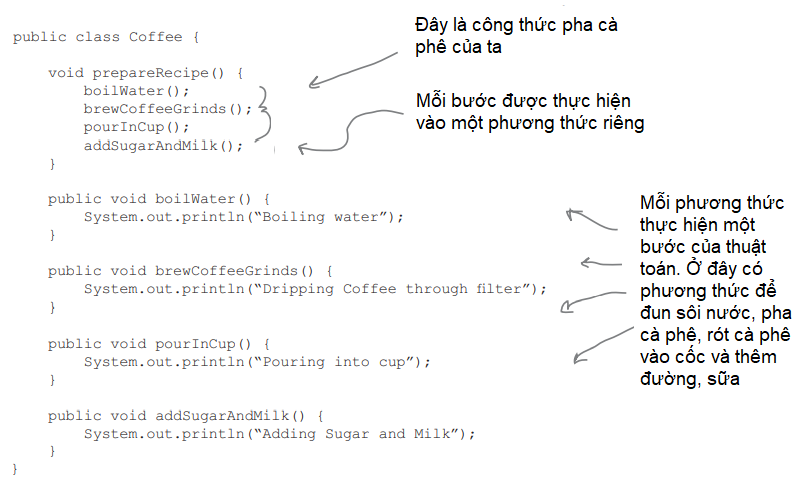
\includegraphics[width=\textwidth]{fig/Template/Coffee.png}/
\end{figure}\\[0.1in]

Trà:
\begin{figure}[!htb]
    \centering
    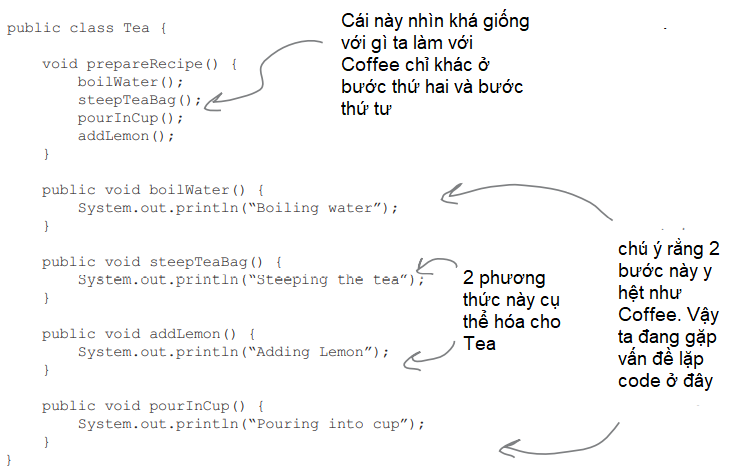
\includegraphics[width=\textwidth]{fig/Template/Tea.png}/
\end{figure}

Rõ ràng có thể thấy code bị dư thừa và lặp lại khá nhiều. Ta phải hạn chế bằng cách nhóm những điểm chung vào một lớp vì cách thức làm cà phê và trà khá tương đồng\\[0.1in]

Lưu ý rằng cả 2 công thức đều được xây dựng trên một thuật toán:
\begin{itemize}
\item Đun sôi nước
\item Dùng nước sôi trích xuất trà / cà phê
\item Đổ thành phẩm vào cốc
\item Thêm gia vị thích hợp
\end{itemize}

Về mặt ý tưởng để cải tiến, ta sẽ tạo một lớp cha tên là \textbf{CaffeineBeverage}. Bên trong lớp này sẽ có một phương thức \textbf{prepareRecipe()} thực hiện thuật toán chung cho cả cà phê lẫn trà\smallskip

Do thuật toán chung có 4 bước nên trong phương thức \textbf{prepareRecipe()} cũng sẽ có 4 phương thức đại diện: \textbf{boilWater()}, \textbf{brew()}, \textbf{pourInCup()}, \textbf{addCondiments()}\smallskip

Do cách trích xuất và thêm gia vị của cà phê, trà là khác nhau nên phương thức \textbf{brew()}, \textbf{addCondiments()} sẽ đánh dấu abstract. Còn lại sẽ được triển khai trong lớp cha
\newpage

Dưới đây là code minh họa cho lớp \textbf{CaffeineBeverage}:

\begin{figure}[!htb]
    \centering
    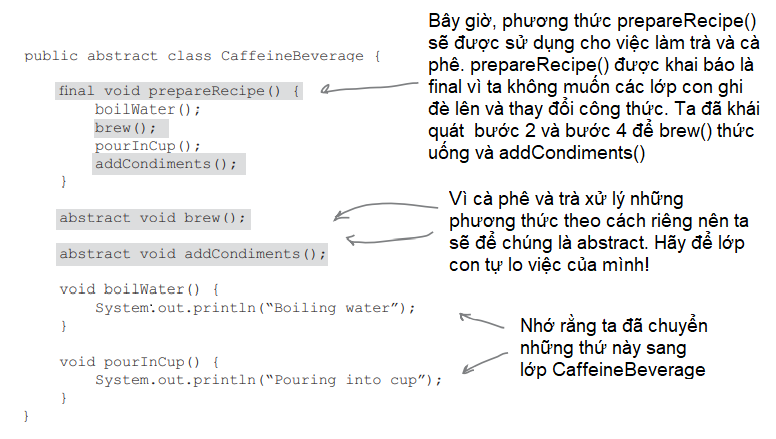
\includegraphics[width=\textwidth]{fig/Template/CaffeineBeverage.png}/
\end{figure}

Đây là code cho 2 lớp \textbf{Tea} và \textbf{Coffee} với cách thiết kế mới:
\begin{figure}[!htb]
    \centering
    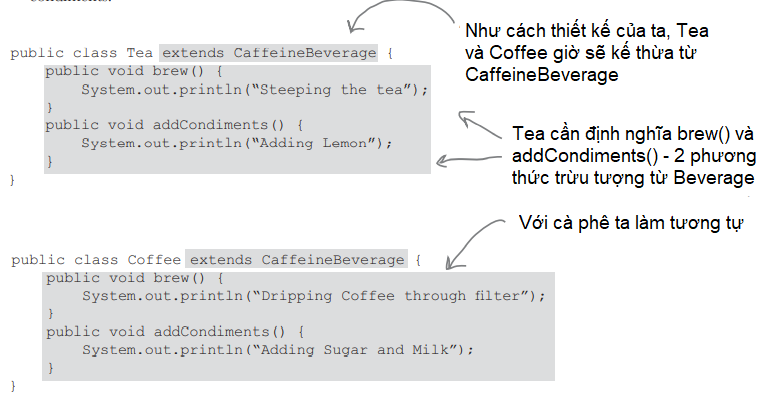
\includegraphics[width=\textwidth]{fig/Template/TeaAndCoffeeNewDesign.png}/
\end{figure}

Tổng kết lại, những gì ta đã làm là cài đặt \textbf{Template Method Pattern}. Phương thức \textbf{prepareRecipe()} được gọi là \textbf{Template Method}\smallskip

Qua ví dụ trên, \textbf{Template Method Pattern} giúp tối đa hóa việc tái sử dụng code giữa các lớp. Hơn nữa, thuật toán sẽ nằm yên một chỗ thuận tiện trong quá trình sửa đổi. Cuối cùng, Template cung cấp một Framework hỗ trợ các loại đồ uống chứa caffeine khác nếu ta muốn cải tiến chương trình sau này. Đó cũng là mục đích sử dụng chính của \textbf{Template Method Pattern}.

\newpage
\section{Định nghĩa và Mô hình cấu trúc}
\subsection{Định nghĩa}

\textbf{Template Method Pattern} định ra khung xương cho thuật toán trong một phương thức, trì hoãn một số bước tới những lớp con. Template Method cho phép những lớp con tự định nghĩa lại một số bước nhất định mà không làm thay đổi cấu trúc thuật toán

\subsection{Mô hình cấu trúc}

Mô hình cấu trúc của Template Method Pattern được mô tả như sau:

\begin{figure}[!htb]
    \centering
    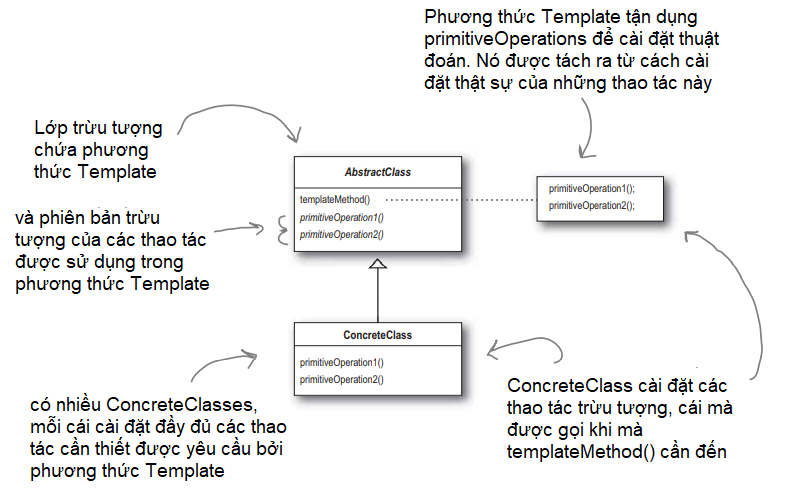
\includegraphics[width=\textwidth]{fig/Template/TemplateDiagram.png}/
\end{figure}

\section{Thực tế}
Template Method Pattern khá là cơ bản đến nỗi nó được thấy ở hầu hết các lớp trừu tượng \\[0.1in]
Dưới đây là những phương thức Template trong bộ thư viện chuẩn của Java:
\begin{itemize}
    \item Tất cả các phương thức không phải trừu tượng của \textbf{java.io.InputStream}, \textbf{java.io.OutputStream}, \textbf{java.io.Reader}, \textbf{java.io.Writer}
    \item Tất cả các phương thức không phải trừu tượng của
    \textbf{java.util.AbstractList}, \textbf{java.util.AbstractSet}, \textbf{java.util.AbstractMap}
\end{itemize}

%=== END OF MM ===
\newpage